\section{Results and Discussions}

\subsection{Experimental Setup}
\label{sec:experimental_setup}

To ensure a fair and direct comparison, we closely follow the experimental methodology of Coconut~\cite{hao2024training}, aligning model architecture, training curriculum, datasets, and optimization settings. This design isolates the impact of the proposed Parallel Continuous Thought (PaCT) architecture from other confounding factors.

All experiments are conducted using GPT-2 Small (124M parameters) as the primary base causal language model, without modifying the underlying Transformer layers. In addition, to evaluate the scalability of our approach across model sizes, we perform experiments using LLaMA-3B and LLaMA-8B as alternative base models. In all cases, the PaCT module is integrated on top of the base model with identical architectural design.

The PaCT module uses a fixed configuration across tasks and model scales. We employ a latent codebook with projection dimension 128 and 4 attention heads for the cross-attention mechanism. Latent synthesis attends to a restricted context consisting of the two most recent hidden states, which serve as keys and values for the codebook queries.

Training follows the multi-stage curriculum paradigm introduced in Coconut, in which explicit language-based reasoning steps are progressively replaced by continuous latent reasoning steps. At each stage, the number of latent steps is increased while the number of language reasoning steps is reduced, until a fully latent reasoning regime is reached. For GSM8k, we first fine-tune the pretrained model for 25 epochs using chain-of-thought supervision, followed by 25 epochs of curriculum-based latent training. For ProntoQA and ProsQA, models are trained for a total of 50 epochs using the same curriculum schedule as Coconut. The maximum number of latent stages is set to 3 for GSM8k and 6 for both ProntoQA and ProsQA.

Across all experiments, we use the AdamW optimizer with a learning rate of $1\times10^{-4}$, weight decay of 0.01, and an effective batch size of 128. We evaluate on three standard reasoning benchmarks: GSM8k for mathematical reasoning, ProntoQA for deductive logical reasoning, and ProsQA for proof-oriented reasoning. Following prior work, the continuous thought parameter $c_{\text{thought}}$ is set to 2 for GSM8k and to 1 for both ProntoQA and ProsQA. All experiments are conducted on a single node with 4 GPUs, matching the hardware configuration used in the Coconut baseline.

%%%%%%%%%%%%%%%%%%%%%%%%%%%%%%%%%%%%%%%%
%%SoTA Table
%%%%%%%%%%%%%%%%%%%%%%%%%%%%%%%%%%%%%%%%

% \begin{table*}[t]
% \centering
% \tiny
% \begin{tabular}{lcccccccccccc}
% \toprule
% \multirow{2}{*}{Method} 
% & \multicolumn{3}{c}{GSM8k} 
% & \multicolumn{3}{c}{ProntoQA} 
% & \multicolumn{3}{c}{ProsQA} \\
% \cmidrule(lr){2-4} 
% \cmidrule(lr){5-7} 
% \cmidrule(lr){8-10} 
% \cmidrule(lr){11-13}
% & Acc. (\%) & Train Time & Infer Time (s)
% & Acc. (\%) & Train Time & Infer Time (s)
% & Acc. (\%) & Train Time & Infer Time (s)\\
% \midrule

% CoT 
% & 42.9 $\pm$ 0.2 & 2.90 & 0.26
% & 98.8 $\pm$ 0.8 & 0.55 & 0.85
% & 77.5 $\pm$ 1.9 & 0.91 & 0.47 \\

% No-CoT 
% & 16.5 $\pm$ 0.5 & 2.18 & 0.020
% & 93.8 $\pm$ 0.7 & 0.90 & 0.020
% & 76.7 $\pm$ 1.0 & 1.54 & 0.050\\

% Pause Token 
% & 16.4 $\pm$ 1.8 & 2.47 & 0.023
% & 77.7 $\pm$ 21.0 & 1.11 & 0.025
% & 75.9 $\pm$ 0.7 & 1.02 & 0.055\\

% iCoT 
% & 30.0$^{*}$ & 2.47 & 0.020
% & 99.8 $\pm$ 0.3 & 1.11 & 0.020
% & 98.2 $\pm$ 0.3 & 1.02 & 0.050\\

% \midrule

% Coconut 
% & 32.0 $\pm$ 1.5 & 15.40 & 0.0307
% & 99.8 $\pm$ 0.2 & 2.11 & 0.0661
% & 97.0 $\pm$ 0.3 & 6.42 & 0.0870\\

% \quad w/o curriculum 
% & 14.4 $\pm$ 0.8 & 9.24 & 0.0307
% & 52.4 $\pm$ 0.4 & 1.27 & 0.0661
% & 76.1 $\pm$ 0.2 & 7.12 & 0.0870\\

% \quad w/o thought 
% & 21.6 $\pm$ 0.5 & 2.47 & 0.020
% & 99.9 $\pm$ 0.1 & 1.11 & 0.020
% & 95.5 $\pm$ 1.1 & 1.02 & 0.050\\

% \quad pause as thought 
% & 24.1 $\pm$ 0.7 & 2.47 & 0.023
% & 100.0 $\pm$ 0.1 & 1.11 & 0.025
% & 96.6 $\pm$ 0.8 & 1.02 & 0.055 \\

% \midrule

% \textbf{Codebook} 
% & \textbf{34.4} $\pm$ 0.1 & 3.30 & \textbf{0.0285}
% & \textbf{100.0} $\pm$ 0.1 & 0.65 & \textbf{0.0614}
% & \textbf{98.67} $\pm$ 0.2 & 1.58 & \textbf{0.0808} \\

% \quad w/o curriculum 
% & 26.2 $\pm$ 0.2 & 4.20 & 0.0285
% & 58.0 $\pm$ 0.1 & 1.73 & 0.0614
% & 82.3 & 2.24 & 0.0808 \\
% \bottomrule
% \end{tabular}
% \caption{Performance--efficiency comparison across GSM8k, ProntoQA, ProsQA.
% CoT training times are measured.
% Training times for other methods are extrapolated from CoT based on curriculum structure, sequence length,
% and number of forward passes.
% Inference times follow the conventions described in the text.}
% \label{tab:main_results}
% \end{table*}

%%%%%%%%%%%%%%%%%%%%%%%%%%%%%%%%%%%%%%%%%%%%%%%%%%%%%%
%%%SoTA Table V1
% \begin{table*}[t]
% \centering
% \tiny
% \begin{tabular}{lcccccccccccc}
% \toprule
% \multirow{2}{*}{Method} 
% & \multicolumn{3}{c}{GSM8k} 
% & \multicolumn{3}{c}{ProntoQA} 
% & \multicolumn{3}{c}{ProsQA} \\
% \cmidrule(lr){2-4} 
% \cmidrule(lr){5-7} 
% \cmidrule(lr){8-10} 
% \cmidrule(lr){11-13}
% & Acc. (\%) & Train Time & Infer Time (s)
% & Acc. (\%) & Train Time & Infer Time (s)
% & Acc. (\%) & Train Time & Infer Time (s)\\
% \midrule

% CoT 
% & 42.9 $\pm$ 0.2 & 2.90 & 0.26
% & 98.8 $\pm$ 0.8 & 0.55 & 0.85
% & 77.5 $\pm$ 1.9 & 0.91 & 0.47 \\

% No-CoT 
% & 16.5 $\pm$ 0.5 & 2.18 & 0.020
% & 93.8 $\pm$ 0.7 & 0.41 & 0.020
% & 76.7 $\pm$ 1.0 & 0.68 & 0.050\\

% Pause Token 
% & 16.4 $\pm$ 1.8 & 2.47 & 0.023
% & 77.7 $\pm$ 21.0 & 0.47 & 0.025
% & 75.9 $\pm$ 0.7 & 0.77 & 0.055\\

% iCoT 
% & 30.0$^{*}$ & 2.47 & 0.020
% & 99.8 $\pm$ 0.3 & 0.47 & 0.020
% & 98.2 $\pm$ 0.3 & 0.77 & 0.050\\

% \midrule

% Coconut 
% & 32.0 $\pm$ 1.5 & 15.40 & 0.0307
% & 99.8 $\pm$ 0.2 & 2.11 & 0.0661
% & 97.0 $\pm$ 0.3 & 6.42 & 0.0870\\

% \quad w/o curriculum 
% & 14.4 $\pm$ 0.8 & 9.24 & 0.0307
% & 52.4 $\pm$ 0.4 & 1.27 & 0.0661
% & 76.1 $\pm$ 0.2 & 7.12 & 0.0870\\

% \quad w/o thought 
% & 21.6 $\pm$ 0.5 & 2.47 & 0.020
% & 99.9 $\pm$ 0.1 & 1.11 & 0.020
% & 95.5 $\pm$ 1.1 & 1.02 & 0.050\\

% \quad pause as thought 
% & 24.1 $\pm$ 0.7 & 2.47 & 0.023
% & 100.0 $\pm$ 0.1 & 1.11 & 0.025
% & 96.6 $\pm$ 0.8 & 1.02 & 0.055 \\

% \midrule

% \textbf{PaCT} 
% & \textbf{34.4} $\pm$ 0.1 & 3.30 & \textbf{0.0285}
% & \textbf{100.0} $\pm$ 0.1 & 0.65 & \textbf{0.0614}
% & \textbf{98.67} $\pm$ 0.2 & 1.58 & \textbf{0.0808} \\

% \quad w/o curriculum 
% & 26.2 $\pm$ 0.2 & 4.20 & 0.0285
% & 58.0 $\pm$ 0.1 & 1.73 & 0.0614
% & 82.3 & 2.24 & 0.0808 \\
% \bottomrule
% \end{tabular}
% \caption{Performance--efficiency comparison across GSM8k, ProntoQA, ProsQA.
% CoT training times are measured.
% Training times for other methods are extrapolated from CoT based on curriculum structure, sequence length,
% and number of forward passes.
% Inference times follow the conventions described in the text.}
% \label{tab:main_results}
% \end{table*}
%%%%%%%%%%%%%%%%%%%%%%%%%%%%%%%%%%%%%%%%%%%%%%%%%%%%%%%%%%%%

%%%%%%%%%%%%%%%%%%%%%%%%%%%%%%%%%%%%%%
%%Table V2
\begin{table*}[t]
\centering

\begin{tabular}{lcccccc}
\toprule
\multirow{2}{*}{Method} 
& \multicolumn{2}{c}{GSM8k} 
& \multicolumn{2}{c}{ProntoQA} 
& \multicolumn{2}{c}{ProsQA} \\
\cmidrule(lr){2-3} 
\cmidrule(lr){4-5} 
\cmidrule(lr){6-7} 
& Acc. (\%) & Train Time(Hrs)
& Acc. (\%) & Train Time(Hrs)
& Acc. (\%) & Train Time(Hrs) \\
\midrule

CoT 
& 42.9 $\pm$ 0.2 & 2.90
& 98.8 $\pm$ 0.8 & 0.55
& 77.5 $\pm$ 1.9 & 0.91 \\

No-CoT 
& 16.5 $\pm$ 0.5 & 2.18
& 93.8 $\pm$ 0.7 & 0.41
& 76.7 $\pm$ 1.0 & 0.68 \\

Pause Token 
& 16.4 $\pm$ 1.8 & 2.47
& 77.7 $\pm$ 21.0 & 0.47
& 75.9 $\pm$ 0.7 & 0.77 \\

iCoT 
& 30.0$ & 2.47
& 99.8 $\pm$ 0.3 & 0.47
& 98.2 $\pm$ 0.3 & 0.77 \\

\midrule

Coconut 
& 32.0 $\pm$ 1.5 & 15.40
& 99.8 $\pm$ 0.2 & 2.11
& 97.0 $\pm$ 0.3 & 6.42 \\



\textbf{PaCT} 
& \textbf{34.4} $\pm$ 0.1 & \textbf{3.30}
& \textbf{100.0} $\pm$ 0.1 & \textbf{0.65}
& \textbf{98.67} $\pm$ 0.2 & \textbf{1.58} \\

\bottomrule
\end{tabular}
\caption{Performance--training efficiency comparison across GSM8k, ProntoQA, and ProsQA.
CoT training times(in Hrs) are measured directly.
Training times for other methods are extrapolated from CoT based on curriculum structure,
sequence length, and number of forward passes.}
\label{tab:main_results}
\end{table*}
%%%%%%%%%%%%%%%%%%%%%%%%%%%%%%%%%%%%%


% \begin{table*}[t]
% \centering
% %\resizebox{\columnwidth}{!}{
% \begin{tabular}{lcccccc}
% \toprule
% \multirow{2}{*}{Method} 
% & \multicolumn{2}{c}{GSM8k} 
% & \multicolumn{2}{c}{ProntoQA} 
% & \multicolumn{2}{c}{ProsQA} \\
% \cmidrule(lr){2-3} \cmidrule(lr){4-5} \cmidrule(lr){6-7}
% & Acc. (\%) & \# Tokens & Acc. (\%) & \# Tokens & Acc. (\%) & \# Tokens \\
% \midrule
% CoT & 42.9 $\pm$ 0.2 & 25.0 & 98.8 $\pm$ 0.8 & 92.5 & 77.5 $\pm$ 1.9 & 49.4 \\
% No-CoT & 16.5 $\pm$ 0.5 & 2.2 & 93.8 $\pm$ 0.7 & 3.0 & 76.7 $\pm$ 1.0 & 8.2 \\
% iCoT & 30.0$^{*}$ & 2.2 & 99.8 $\pm$ 0.3 & 3.0 & 98.2 $\pm$ 0.3 & 8.2 \\
% Pause Token & 16.4 $\pm$ 1.8 & 2.2 & 77.7 $\pm$ 21.0 & 3.0 & 75.9 $\pm$ 0.7 & 8.2 \\
% \midrule
% Coconut & 34.2 $\pm$ 1.5 & 8.2 & 99.8 $\pm$ 0.2 & 9.0 & 97.0 $\pm$ 0.3 & 14.2 \\
% \quad w/o curriculum & 14.4 $\pm$ 0.8 & 8.2 & 52.4 $\pm$ 0.4 & 9.0 & 76.1 $\pm$ 0.2 & 14.2 \\
% \quad w/o thought & 21.6 $\pm$ 0.5 & 2.3 & 99.9 $\pm$ 0.1 & 3.0 & 95.5 $\pm$ 1.1 & 8.2 \\
% \quad pause as thought & 24.1 $\pm$ 0.7 & 2.2 & 100.0 $\pm$ 0.1 & 3.0 & 96.6 $\pm$ 0.8 & 8.2 \\
% \midrule
% \textbf{PaCT} & \textbf{34.8} $\pm$ 0.1 & 8.2 & \textbf{100.0} $\pm$ 0.1 & 9.0 & \textbf{98.67} $\pm$ 0.2 & 14.2 \\
% \quad w/o curriculum & - & - & - & - & - & - \\
% \quad w/o thought & - & - & - & - & - & - \\
% \quad pause as thought & - & - & - & - & - & - \\
% \bottomrule
% \end{tabular}
% %}
% \caption{Performance comparison across GSM8k, ProntoQA, and ProsQA.}
% \label{tab:main_results}
% \end{table*}

% \begin{table*}[t]
% \centering
% %\resizebox{\columnwidth}{!}{
% \begin{tabular}{l l c c c}
% \toprule
% Method & Dataset & Accuracy (\%) & Training Time (hrs) & \# Stages \\
% \midrule
% iCoT & GSM8k & 30.00 & 11.65 (assumed) & 3 \\
% Coconut & GSM8k & 34.20 & 15.40 & 3 \\
% PaCT & GSM8k & \textbf{34.80} & \textbf{3.60 } & 3 \\
% \midrule
% iCoT & ProverQA & 83.30 (assumed) & 6.35 (assumed) & 6 \\
% Coconut & ProverQA & 86.20 & 8.40 & 6 \\
% PaCT & ProverQA & 86.20 & \textbf{0.93} & 6 \\
% \bottomrule
% \end{tabular}
% %}
% \caption{Training time comparison between Coconut and PaCT methods across datasets. PaCT achieves comparable accuracy with significantly reduced training time.}
% \label{tab:time_comparison}
% \end{table*}

\subsection{Parallel Latent Reasoning Improves Computational Efficiency}
\label{sec:efficiency}

Table~\ref{tab:main_results} reports accuracy, training time, and inference time for Parallel Continuous Thought (PaCT) and prior methods on GSM8k, ProntoQA, and ProsQA. Across all evaluated benchmarks, PaCT consistently maintains strong reasoning performance while substantially reducing computational cost compared to sequential continuous thought approaches.

Changing the sequential nature of unrolling lalents into a slot wise parallel latent generation via the PaCT module leads to siginificant reductions in training time. On GSM8k, training time decreases from 15.4 hours with Coconut to 3.3 hours with PaCT, corresponding to nearly a $5\times$ speedup. Similar improvements are observed on ProsQA, where training time is reduced from 13.6 hours to 1.49 hours. 



Importantly, the efficiency gains provided by PaCT do not come at the cost of reasoning quality. Across GSM8k, ProntoQA, and ProsQA, PaCT matches or exceeds the accuracy of Coconut and other strong baselines while requiring substantially less computation. This demonstrates that parallel latent reasoning preserves the benefits of continuous thought while removing its primary computational bottleneck, enabling more efficient scaling to larger models and more complex reasoning tasks. Figure \ref{fig:inference_time} compares inference time across models.


\begin{table}[t]
    \centering
    \small
    \caption{Performance and training cost (Time in Hrs) across model sizes}
    \label{tab:performance_training}
\begin{tabular}{lcccccc}
\toprule
 &  & \multicolumn{2}{c}{Coconut} & \multicolumn{2}{c}{PaCT} \\
\cmidrule(lr){3-4} \cmidrule(lr){5-6}
Model & Params & Acc & Time(Hrs) & Acc & Time(Hrs) \\
\midrule
LLaMA 3.2 & 3B & 31.7 & 51.5 & \textbf{36.4} & 11.02 \\
LLaMA 3   & 8B & 43.6 & 105.9 & \textbf{43.6} & 22.68 \\
\bottomrule
\end{tabular}
\end{table}

% \begin{table*}[t]
%     \centering
%     \caption{Training time for PaCT}
%     \label{tab:inference_time}
%     \begin{tabular}{lcccc}
%         \toprule
%         \textbf{Model} & \textbf{Dataset} & \textbf{Accuracy} & \textbf{Training Time (hrs)} \\
%         \midrule
%         LLaMA 3B & ProsQA   & 100\% & 2.71 \\
%         LLaMA 3B & ProntoQA & 100\% & 1.08 \\
%         LLaMA 8B & ProsQA   & 100\% & 4.60 \\
%         LLaMA 8B & ProntoQA & 100\% & 2.03 \\
%         \bottomrule
%     \end{tabular}
% \end{table*}

\subsection{Every latent stage contributes to performance}

\begin{figure}[t]
    \centering
    \begin{subfigure}[b]{0.48\textwidth}
        \centering
        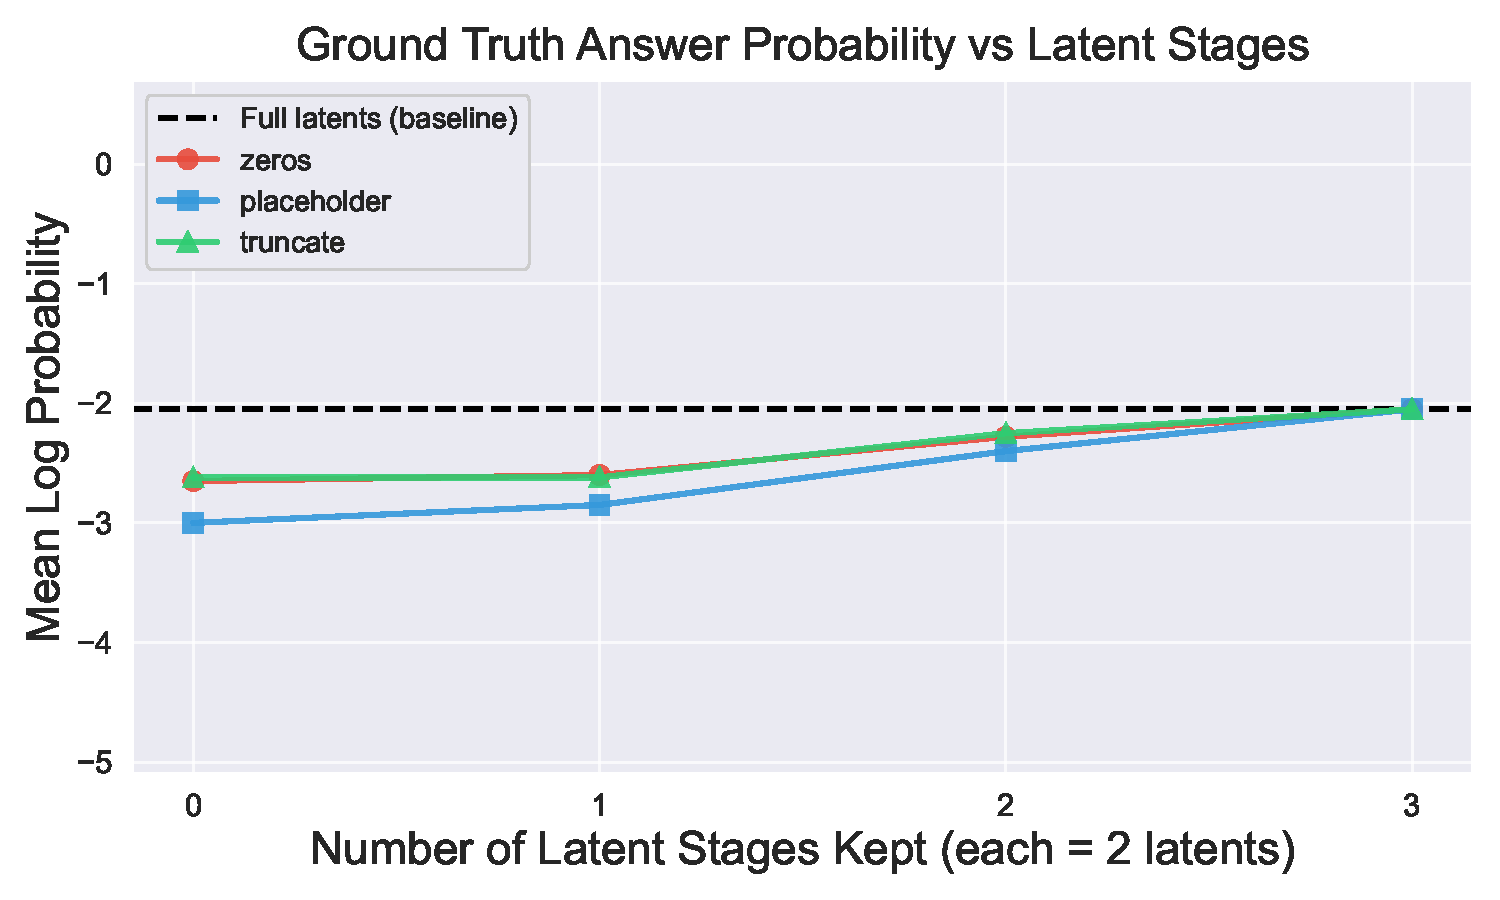
\includegraphics[width=\textwidth]{imgs/ablation_log_probs.pdf}
        \caption{Absolute log-probabilities}
        \label{fig:ablation_log_probs}
    \end{subfigure}
    \hfill
    
    \caption{Latent token analysis. (a) Mean log-probability of the generated answer as a function of latent stages retained, under three ablation methods. (b) Log-probability drop relative to the full-latent baseline. Both plots show that retaining more latent stages consistently improves model confidence.}
    \label{fig:ablation}
\end{figure}

While our method offers tremendous increases to scalability, the question is whether the model actually benefits from an increased number of latent tokens. A natural way to answer this question is to study the information afforded by the latents and whether they contribute meaningfully to the model's overall performance.

\noindent
We progressively removed latent stages (each containing $c_{\text{thought}}=2$ latent tokens) and measured the resulting change in log-probability of the model's generated token and the expected ground truth token, across 500 validation samples. Three \textit{actions} were applied individually on each latent stage:
\begin{itemize}
    \item Replacing latent embeddings with zero vectors
    \item Replacing latent embeddings with the original placeholder embeddings \textit{before the transformer block}
    \item Truncating the latent positions entirely from the sequence
\end{itemize}

Figures~\ref{fig:ablation_log_probs} presents the results as absolute log-probabilities, revealing a clear monotonic relationship: retaining more latent stages consistently yields higher answer probabilities. 

These results demonstrate that the latent stages actively encode intermediate reasoning states that progressively refine the model's confidence in the final answer, serving as validation that latent stages are individually meaningful.

\subsection{Latent token and latent stage information content}

The stage-wise resynthesis of latent tokens in PaCT as detailed in \ref{sec:latent_deliberation} allows latent tokens to be derived from context, without direct dependence on previous latent values leading to functionally independent latent tokens in across stages. Thus we hypothesize that the latent tokens in PaCT are more information dense than those of Coconut. To mechanistically compare the quality of latent tokens and stages between PaCT and Coconut, we analyzed the similarity of latent hidden states in the last stage after transformer processing for samples with three reasoning stages. We computed pairwise cosine similarities between the hidden representations at latent positions and additionally performed a swap experiment where we exchanged the two latent tokens and measured the effect on model outputs. This analysis was conducted for both PaCT and Coconut and summarize our findings in \ref{tab:latent_similarity}.

\begin{table}[H]
\centering
\caption{Latent representation similarity analysis. PaCT produces dissimilar stages and similar within-stage latent tokens, while Coconut produces dissimilar within-stage latent tokens and similar stages.}
\label{tab:latent_similarity}
\small
\begin{tabular}{lcc}
\toprule
{Metric} & {PaCT} & {Coconut} \\
\midrule
Within-stage cosine similarity & $0.99 \pm 0.01$ & $0.30 \pm 0.17$ \\
Cross-stage cosine similarity & $0.31 \pm 0.21$ & $0.63 \pm 0.14$ \\
% Drop in Acc after L4$\leftrightarrow$L5 swap & $1.2\%$ & $19.4\%$ \\
% Within-stage swap $\Delta$log-prob & $0.00$ & $0.23$ \\
\bottomrule
\end{tabular}
\end{table}

We observe the following two distinct opposing trends between PaCT and Coconut which lead us to two further conclusions detailed next:
\begin{itemize}
    \item Within-stage latent tokens exhibit near-perfect similarity in their hidden representations in PaCT, indicating they encode essentially identical information. In Coconut however, the latent tokens are far less similar indicating that \textbf{both} latent tokens are required for effective reasoning.
    \item Cross-stage latent tokens show substantially lower similarity in PaCT, indicating that \textbf{different reasoning stages capture distinct information}. This is unlike in Coconut where cross-stage latent token similarity is far higher showcasing the inability of different latent stages to capture meaningfully different information.
    % \item The swap experiment confirms functional interchangeability of latent tokens in PaCT. Exchanging latent tokens produces no meaningful change in output log-probability. However, in Coconut there is a significant drop in performance indicating positional dissimilarity of tokens
\end{itemize}

% With this observation, we draw the following two important formative conclusions:

\subsubsection{Depth vs.\ Width: More Stages Outperforms More Latents Per Stage}

\begin{table}[H]
% \begin{table}[h]
\centering
\small
%\resizebox{\columnwidth}{!}{
\begin{tabular}{l l c c}
\toprule
Method & Dataset & Accuracy (\%) & \# Stages \\
\midrule
Coconut & GSM8k & 34.2 & 3 \\
PaCT & GSM8k & 34.8 & 3 \\
PaCT & GSM8k & 36.6 & 6 \\
PaCT & GSM8k & \textbf{37.2} & \textbf{8} \\
\bottomrule
\end{tabular}

\caption{Scaling behavior with increasing number of training stages on GSM8k with $c_{\text{thought}}=2$. Accuracy improves as PaCT scales to more stages.}
\label{tab:stage_scaling}
\end{table}



Having established the increased information associated with more latent tokens, a question that arises is whether to increase \emph{depth} (more reasoning stages) or \emph{width} (more latent tokens per stage, i.e., larger $c_{\text{thought}}$). The analysis of \ref{tab:latent_similarity} directly provides an answer to this question in that since latent tokens of a single stage in PaCT show similarity which is \textbf{not} present across stages, computational resources are better allocated to deeper reasoning chains rather than wider parallel representations within each step. To showcase the scaling of performance with increasing stages, we ablate on increasing reasoning stages and observe an expected improvement in performance as summarized in \ref{tab:stage_scaling}.

% These results provide a mechanistic explanation for why increasing depth yields better scaling than increasing width. Latents within the same stage are encode identical information while each new stage captures genuinely distinct representations, as evidenced by their low cross-stage similarity. 
% We therefore conclude that computational resources are better allocated to deeper reasoning chains rather than wider parallel representations within each step. 

\subsubsection{Quality of latent stages and tokens}

We observe that the quality of latent tokens and stages is more information rich in PaCT than Coconut. Low cross stage similarity in PaCT evidences the learning of more distinct reasoning information. Furthermore, we confirm the improved quality of latent tokens in PaCT by comparing the performance of PaCT with $c_{\text{thought}}=1$ and Coconut with $c_{\text{thought}}=2$ and $S=3$ latent stages in each, summarized below:

\begin{table}[H]
    \centering
    \small
    \caption{Single latent PaCT vs dual latent Coconut on GSM8k}
    \label{tab:1v2}
    \begin{tabular}{lcccc}
        \toprule
        {Model} & {$c_{\text{thought}}$} &{Eval accuracy}\\
        \midrule
        PaCT & 1 & 33.20 \\
        Coconut & 2 & 32.00 \\
        \bottomrule
    \end{tabular}
\end{table}


\subsubsection{Test time latent token truncation}
As a further experiment we observe the effect of test time truncation of one latent in each stage from PaCT trained with $c_{\text{thought}}=2$ and $S=3$ latent stages as shown in \ref{tab:latent_redundancy}. While the drop in accuracy observed on truncation is not significant further showcasing the similarity of latent tokens within a stage, the performance of this method of inference is inferior to directly training the model on $c_{\text{thought}}=1$ (see \ref{tab:1v2}). Thus training a model with greater per stage latent tokens and speeding up inference by dropping latent tokens is not an advisable strategy.

\begin{table}[H]
    \centering
    \small
    \caption{Accuracy when keeping only 1 of 2 latents per stage.}
    \label{tab:latent_redundancy}
    \begin{tabular}{lccc}
        \toprule
        {Configuration} & {\# Latents} & {Accuracy} \\
        % & \textbf{$\Delta$} \\
        \midrule
        Full model & 6 & 34.4\% \\
        % & --- \\
        First of each (L0, L2, L4) & 3 & 31.6\% \\
        % & $-$2.8\% \\
        Second of each (L1, L3, L5) & 3 & 31.6\% \\
        % & $-$2.8\% \\
        \bottomrule
    \end{tabular}
\end{table}

\subsection{Latent Token Decoding Analysis}
\label{sec:latent_decoding}

% \begin{table}[h]
% \centering
% \caption{Last-stage latent confidence (top-1 probability at $L_5$) for correct vs.\ incorrect predictions.}
% \label{tab:latent_confidence}
% \begin{tabular}{lcc}
% \toprule
% & \textbf{Correct} ($n$=166) & \textbf{Incorrect} ($n$=334) \\
% \midrule
% Mean $\pm$ Std & $0.712 \pm 0.294$ & $0.268 \pm 0.249$ \\
% \bottomrule
% \end{tabular}
% \end{table}

% \begin{table}[t]
% \centering
% \small
% \caption{Accuracy across datasets and number of stages}
% \label{tab:results}
% \begin{tabular}{lcc}
% \hline
% {Dataset} & {Stages} & {Accuracy (\%)} \\
% \hline
% ProsQA   & 2 & 88.33 \\
% ProsQA   & 4 & 96.67 \\
% ProsQA   & 6 & 98.67 \\
% ProsQA   & 8 & 99.33 \\
% \hline
% ProntoQA & 2 & 55.5  \\
% ProntoQA & 4 & 68.2  \\
% ProntoQA & 6 & 100   \\
% ProntoQA & 8 & 100   \\
% \hline
% GSM8k    & 2 & 33.4  \\
% GSM8k    & 4 & 36.2  \\
% GSM8k    & 6 & 36.6  \\
% GSM8k    & 8 & 37.2  \\
% \hline
% \end{tabular}
% \end{table}


\colorbox{red}{PLOT FOR TABLE 7 @PRakash bhaiya}
\begin{figure}[h!]
  \centering
  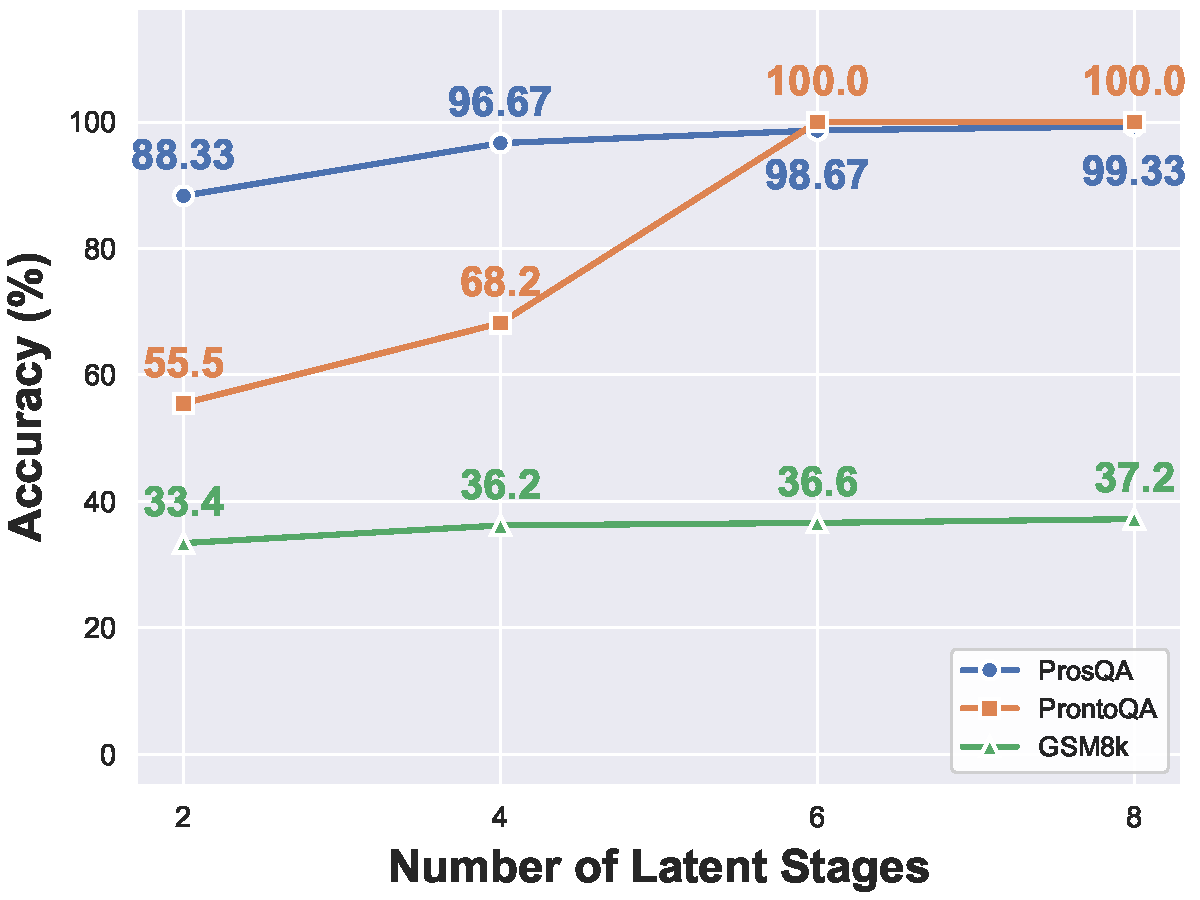
\includegraphics[width=\linewidth]{imgs/table_seven_styled_values.pdf}
      \caption{Accuracy across datasets and number of stages}
  \label{fig:accuracy_and_latent_stages}
\end{figure}

% \begin{table*}[t]
% % \begin{table}[h]
% \centering
% \caption{Last-stage latent confidence (top-1 probability at final latent) for correct vs.\ incorrect predictions.}
% \label{tab:latent_confidence}
% \begin{tabular}{lcccc}
% \toprule
% & \multicolumn{2}{c}{\textbf{Ours}} & \multicolumn{2}{c}{\textbf{Base Coconut}} \\
% \cmidrule(lr){2-3} \cmidrule(lr){4-5}
% & Correct & Incorrect & Correct & Incorrect \\
% \midrule
% % $n$ & 166 & 334 & 160 & 340 \\
% Mean $\pm$ Std & $0.680 \pm 0.315$ & $0.257 \pm 0.223$ & $0.744 \pm 0.244$ & $0.312 \pm 0.232$ \\
% \bottomrule
% \end{tabular}
% \end{table*}

\begin{table}[H]
\centering
\small
\caption{Last-stage latent confidence (top-1 probability at final latent) for correct vs.\ incorrect predictions.}
\label{tab:latent_confidence}
\begin{tabular}{lcc}
\toprule
{Model} & {Correct} & {Incorrect} \\
\midrule
PaCT          & $0.680 \pm 0.315$ & $0.257 \pm 0.223$ \\
Coconut  & $0.744 \pm 0.244$ & $0.312 \pm 0.232$ \\
\bottomrule
\end{tabular}
\end{table}


To understand what information latent tokens encode, we project each latent embedding back into vocabulary space by extracting the top predicted tokens at each latent position after the transformer pass. This allows us to trace how the model's internal reasoning evolves across latent iterations. We present numerical confidence scores of the final latent token for correct and incorrect solutions over the validation split in ~\ref{tab:latent_confidence} and one representative example for a question the model got right and one it got wrong below, showing the question, ground truth chain-of-thought, model prediction, and the decoded latent trajectory. Further examples are provided in the supplementary.

% \vspace{1em}
% \noindent\fbox{\parbox{0.97\textwidth}{
% \textbf{Example 1} \hfill \textcolor{green!60!black}{\textbf{Correct}} \\[0.5em]
% \textbf{Question:} A set of 7 spoons costs \$21. If each spoon would be sold separately, how much would 5 spoons cost? \\[0.3em]
% \textbf{Ground Truth CoT:} $21 \div 7 = 3$ \quad$\rightarrow$\quad $5 \times 3 = 15$ \\[0.3em]
% \textbf{Predicted:} 15 \quad \textbf{GT:} 15 \\[0.5em]
% \begin{tabular}{c|cccccc}
% & L0 & L1 & L2 & L3 & L4 & L5 \\
% \hline
% Token & \textbf{3} & \textbf{3} & \textbf{15} & \textbf{15} & \textbf{15} & \textbf{15} \\
% Prob & 62\% & 66\% & 37\% & 60\% & 84\% & 92\% \\
% \end{tabular} \\[0.3em]
% \textit{Interpretation:} L0--L1 encode the intermediate unit price (3), then L2--L5 converge to the final answer (15).
% }}



% \vspace{1em}
% \noindent\fbox{\parbox{0.97\textwidth}{
% \textbf{Example 2} \hfill \textcolor{green!60!black}{\textbf{Correct}} \\[0.5em]
% \textbf{Question:} Travis wants to fly to Australia. The regular tickets cost about \$2000. As Travis is a student, he will get a 30\% discount on this price. How much does he need to pay for his ticket? \\[0.3em]
% \textbf{Ground Truth CoT:} $2000 \times 0.30 = 600$ \quad$\rightarrow$\quad $2000 - 600 = 1400$ \\[0.3em]
% \textbf{Predicted:} 1400 \quad \textbf{GT:} 1400 \\[0.5em]
% \begin{tabular}{c|cccccc}
% & L0 & L1 & L2 & L3 & L4 & L5 \\
% \hline
% Token & 1400 & 1400 & 1400 & 1400 & 1400 & 1400 \\
% Prob & 2.4\% & 5.3\% & 28\% & 41\% & 89\% & 92\% \\
% \end{tabular} \\[0.3em]
% \textit{Interpretation:} The answer emerges early but with low confidence; probability sharpens dramatically from 2\% to 92\% across stages.
% }}



% \vspace{1em}
% \noindent\fbox{\parbox{0.97\textwidth}{
% \textbf{Example 3} \hfill \textcolor{green!60!black}{\textbf{Correct}} \\[0.5em]
% \textbf{Question:} Kenny played basketball last week. He ran for twice as long as he played basketball, and he practiced on the trumpet for twice as long as he ran. If he practiced on the trumpet for 40 hours, how many hours did Kenny play basketball? \\[0.3em]
% \textbf{Ground Truth CoT:} $40 \div 2 = 20$ \quad$\rightarrow$\quad $20 \div 2 = 10$ \\[0.3em]
% \textbf{Predicted:} 10 \quad \textbf{GT:} 10 \\[0.5em]
% \begin{tabular}{c|cccccc}
% & L0 & L1 & L2 & L3 & L4 & L5 \\
% \hline
% Token & \textbf{20} & \textbf{20} & \textbf{10} & \textbf{10} & \textbf{10} & \textbf{10} \\
% Prob & 4.7\% & 6.8\% & 15\% & 31\% & 95\% & 94\% \\
% \end{tabular} \\[0.3em]
% \textit{Interpretation:} Clear two-step reasoning---L0--L1 encode the intermediate (20 = running time), L2--L5 compute the final answer (10).
% }}
\begin{figure}[H]
\centering
\fbox{%
\parbox{0.97\columnwidth}{
\textbf{Example 1} \hfill \textcolor{green!60!black}{\textbf{Correct}} \\[0.5em]
\textbf{Question:} Kenny played basketball last week. He ran for twice as long as he played basketball, and he practiced on the trumpet for twice as long as he ran. If he practiced on the trumpet for 40 hours, how many hours did Kenny play basketball? \\[0.3em]
\textbf{Ground Truth CoT:} $40 \div 2 = 20$ \quad$\rightarrow$\quad $20 \div 2 = 10$ \\[0.3em]
\textbf{Predicted:} 10 \quad \textbf{GT:} 10 \\[0.5em]
\begin{tabular}{c|cccccc}
& L0 & L1 & L2 & L3 & L4 & L5 \\
\hline
Token & \textbf{20} & \textbf{20} & \textbf{10} & \textbf{10} & \textbf{10} & \textbf{10} \\
Prob & 4.7\% & 6.8\% & 15\% & 31\% & 95\% & 94\% \\
\end{tabular} \\[0.3em]
\textit{Interpretation:} Clear two-step reasoning---L0--L1 encode the intermediate (20 = running time), L2--L5 compute the final answer (10).
}}
\end{figure}


% \vspace{1em}
% \noindent\fbox{\parbox{0.97\textwidth}{
% \textbf{Example 4} \hfill \textcolor{red}{\textbf{Incorrect}} \\[0.5em]
% \textbf{Question:} John cuts his grass to 2 inches. It grows 0.5 inches per month. When it gets to 4 inches he cuts it back down to 2 inches. It costs \$100 to get his grass cut. How much does he pay per year? \\[0.3em]
% \textbf{Ground Truth CoT:} $4-2=2$ \quad$\rightarrow$\quad $2 \div 0.5 = 4$ months \quad$\rightarrow$\quad $12 \div 4 = 3$ cuts \quad$\rightarrow$\quad $100 \times 3 = 300$ \\[0.3em]
% \textbf{Predicted:} 200 \quad \textbf{GT:} 300 \\[0.5em]
% \begin{tabular}{c|cccccc}
% & L0 & L1 & L2 & L3 & L4 & L5 \\
% \hline
% Token & / & / & 200 & 200 & 200 & 5000 \\
% Prob & 0.5\% & 0.4\% & 6.2\% & 11\% & 5.9\% & 8.5\% \\
% \end{tabular} \\[0.3em]
% \textit{Interpretation:} Model fails to compute cutting frequency. Low, unstable probabilities throughout indicate uncertain reasoning. Final latent diverges entirely.
% }} changed by xhitij to reduce overlap 


% \vspace{1em}
% \noindent\fbox{\parbox{0.97\textwidth}{
% \textbf{Example 5} \hfill \textcolor{red}{\textbf{Incorrect}} \\[0.5em]
% \textbf{Question:} Marcia wants to buy some fruit. Apples cost \$2, bananas cost \$1, and oranges cost \$3. If Marcia buys 12 apples, 4 bananas and 4 oranges, what is the average cost of each piece of fruit? \\[0.3em]
% \textbf{Ground Truth CoT:} $12\times2=24$, $4\times1=4$, $4\times3=12$ \quad$\rightarrow$\quad $24+4+12=40$ \quad$\rightarrow$\quad $40 \div 20 = 2$ \\[0.3em]
% \textbf{Predicted:} 1.33 \quad \textbf{GT:} 2 \\[0.5em]
% \begin{tabular}{c|cccccc}
% & L0 & L1 & L2 & L3 & L4 & L5 \\
% \hline
% Token & 24 & 24 & 4 & 4 & 9 & 9 \\
% Prob & 0.6\% & 0.7\% & 42\% & 40\% & 2.5\% & 5.6\% \\
% \end{tabular} \\[0.3em]
% \textit{Interpretation:} L0--L1 correctly identify apple cost (24), L2--L3 fixate on banana cost (4), but the model fails to aggregate totals correctly.
% }} original, commented by xhitij to reduce overlap
\begin{figure}[H]
\centering
\fbox{%
\parbox{0.97\columnwidth}{
\textbf{Example 2} \hfill \textcolor{red}{\textbf{Incorrect}} \\[0.5em]
\textbf{Question:} Marcia wants to buy some fruit. Apples cost \$2, bananas cost \$1, and oranges cost \$3. If Marcia buys 12 apples, 4 bananas and 4 oranges, what is the average cost of each piece of fruit? \\[0.3em]
\textbf{Ground Truth CoT:} $12\times2=24$, $4\times1=4$, $4\times3=12$ \quad$\rightarrow$\quad $24+4+12=40$ \quad$\rightarrow$\quad $40 \div 20 = 2$ \\[0.3em]
\textbf{Predicted:} 1.33 \quad \textbf{GT:} 2 \\[0.5em]
\begin{tabular}{c|cccccc}
& L0 & L1 & L2 & L3 & L4 & L5 \\
\hline
Token & 24 & 24 & 4 & 4 & 9 & 9 \\
Prob & 0.6\% & 0.7\% & 42\% & 40\% & 2.5\% & 5.6\% \\
\end{tabular} \\[0.3em]
\textit{Interpretation:} L0--L1 correctly identify apple cost (24), L2--L3 fixate on banana cost (4), but the model fails to aggregate totals correctly.
}}
\end{figure}


\vspace{1em}
The examples reveal that correct predictions show clear probability sharpening, while incorrect predictions exhibit diffused confidence. Notably, within-stage latent pairs (L0--L1, L2--L3, L4--L5) consistently decode to identical tokens, confirming their functional redundancy.

\subsection{PaCT Promotes Stable Latent Dynamics}
\label{sec:icr_analysis}

\begin{figure}[h!]
  \centering
  
\includegraphics[width=\linewidth]{imgs/icr_plot.pdf}
  \caption{Layer-wise difference in ICR scores between PaCT and Base Coconut. Negative values indicate lower ICR for PaCT.}
  \label{fig:icr}
\end{figure}
Beyond end-task accuracy and efficiency, an important question is how different is the  \emph{internal dynamics} of the model during reasoning in comparision to the Coconut model. 
To address this question, we analyze the evolution of hidden representations using the Information Contribution to the Residual Stream (ICR) score \cite{zhang2025icr}.


ICR\cite{zhang2025icr}, introduced in prior work as a diagnostic for hallucination and instability in large language models, measures the extent to which a Transformer layer’s residual update deviates from what is explained by attention alone. Lower ICR indicates that a layer primarily redistributes existing contextual information in an attention-aligned manner, whereas higher ICR reflects stronger feedforward-driven updates that introduce new, non-attention-guided information. Sustained elevation of ICR—particularly in middle layers associated with semantic processing—has been shown to correlate with prolonged internal uncertainty and unreliable reasoning dynamics.

Figure~\ref{fig:icr} presents the layer-wise difference in ICR between PaCT and the Coconut model. Across the middle Transformer layers, PaCT consistently exhibits lower ICR in comparision to Coconut, indicating that its internal representations stabilize earlier during reasoning in comparision. This behavior is consistent with the design of PaCT, where latent tokens are re-synthesized stage-wise from context and are grounded by the residual connection coming from question token. As a result, each reasoning stage begins from a grounded, question-conditioned representation rather than accumulating latent history, reducing unnecessary internal rewriting.



\subsection{Effect of Context Length}
\label{subsec:context_length}
\begin{table}[t]
    \centering
    \caption{Effect of number of context tokens used GPT-2 performance on GSM8K}
    \label{tab:gpt2_gsm8k_context}
    \begin{tabular}{lcc}
        \toprule
        \textbf{Model} & \textbf{\# Context tokens} & \textbf{Accuracy (\%)} \\
        \midrule
        GPT-2 & 2   & 34.4 \\
        GPT-2 & 4   & 33.0 \\
        GPT-2 & 8   & 34.4 \\
        GPT-2 & All & 30.6 \\
        \bottomrule
    \end{tabular}
\end{table}

A key design choice in our PaCT is the number of context tokens (\texttt{num\_ctx}) used as key-value inputs to the cross-attention mechanism. We hypothesize that the model primarily relies on the most recent hidden states when generating latent representations, and that providing excessive context may dilute the attention signal and degrade performance.

To validate this hypothesis, we trained models with varying context lengths: \texttt{num\_ctx} $\in \{2, 4, 8, \text{ALL}\}$, where ``ALL'' indicates using the entire prefix hidden states. We then extracted and analyzed the cross-attention weights across all samples in the GSM8K validation set. Two key observations emerge:

\begin{figure}[t]
    \centering
    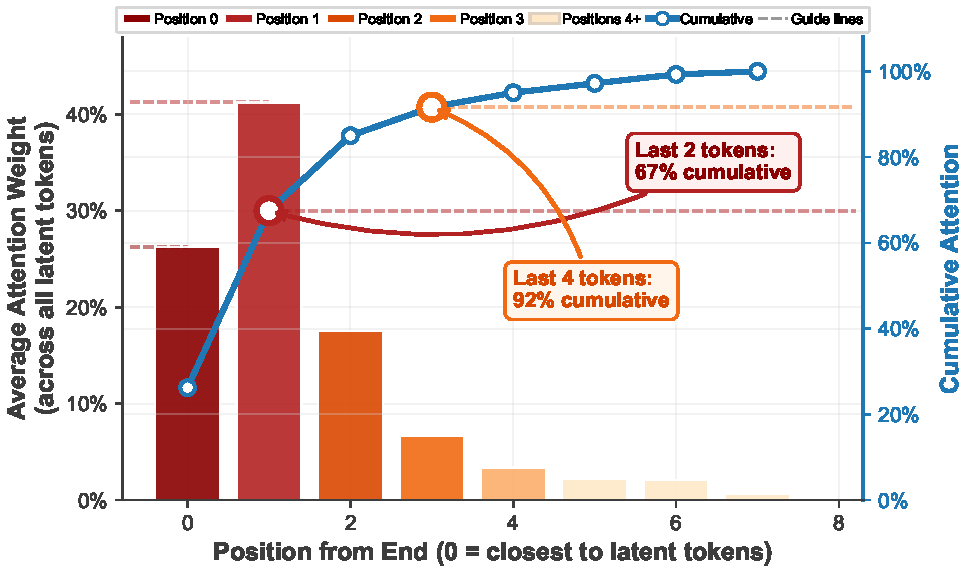
\includegraphics[width=\linewidth]{imgs/cross_attention_bias.pdf}
    \caption{Cross-attention weight distribution across different context length settings. Position 0 represents the \textbf{last} token before the latent tokens, position 1 the \textbf{second-to-last}, and so on. Brighter colors indicate higher attention weights. The model consistently concentrates attention on the last 1-2 positions regardless of available context.}
    \label{fig:attention_heatmap}
\end{figure} 

% \begin{figure}[t]
%     \centering
%     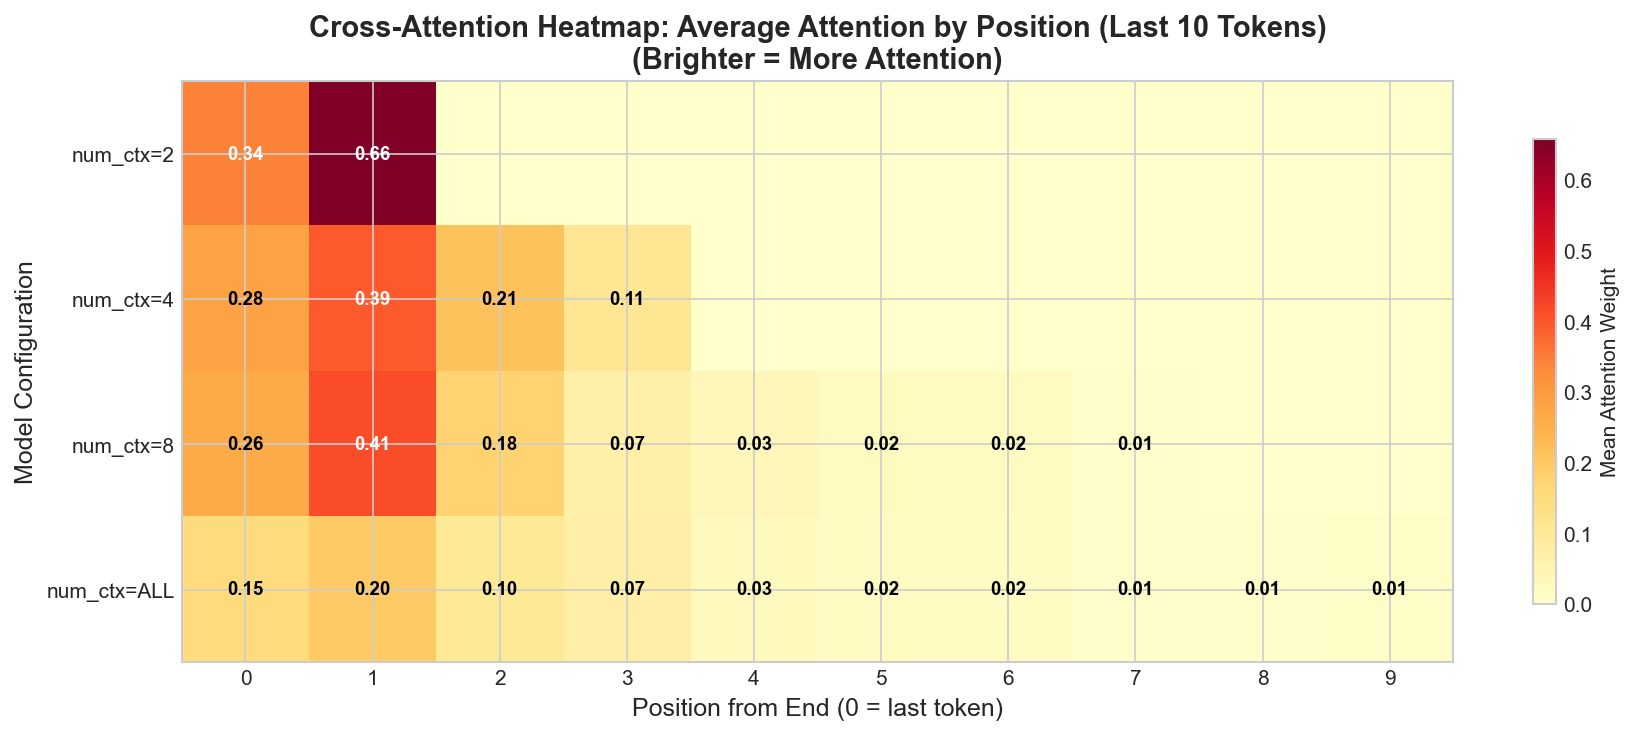
\includegraphics[width=\linewidth]{imgs/attention_heatmap.png}
%     \caption{Cross-attention weight distribution across different context length settings. Position 0 represents the \textbf{last} token before the latent tokens, position 1 the \textbf{second-to-last}, and so on. Brighter colors indicate higher attention weights. The model consistently concentrates attention on the last 1-2 positions regardless of available context.}
%     \label{fig:attention_heatmap}
% \end{figure} 

% \begin{table}[t]
%     \centering
%     \caption{Effect of context length on model accuracy and attention distribution. Attention percentages show mean weights on the last token (Pos 0) and last two tokens (Pos 0+1) across all validation samples.}
%     \label{tab:context_length}
%     \begin{tabular}{lccc}
%         \toprule
%         \textbf{num\_ctx} & \textbf{Accuracy} & \textbf{Attn @ Pos 0} & \textbf{Attn @ Pos 0+1} \\
%         \midrule
%         2   & \textbf{33.2\%} & 34.2\% & 100.0\% \\
%         4   & 31.8\% & 28.2\% & 67.7\% \\
%         8   & 31.4\% & 26.2\% & 67.5\% \\
%         ALL & 30.2\% & 15.1\% & 34.6\% \\
%         \bottomrule
%     \end{tabular}
% \end{table}

\begin{itemize}
    \item \textbf{Attention is concentrated on recency:} As shown in Figure~\ref{fig:attention_heatmap}, regardless of how much context is available, the cross-attention mechanism consistently assigns the highest weights to the most recent positions. Even when given access to the full prefix (up to 170 tokens in some samples), the model places approximately 35\% of its attention on just the last two tokens.

    \item \textbf{More context hurts performance:} Increasing the context length leads to decreased accuracy (refer \ref{tab:gpt2_gsm8k_context}). This suggests that the additional context introduces noise that dilutes the attention signal on the truly relevant recent tokens.
\end{itemize}

% \textbf{Optimal context is minimal.} The best performance is achieved with \texttt{num\_ctx}=2, where the model is forced to focus entirely on the last two hidden states. This validates our architectural choice and demonstrates that for iterative latent generation, recency dominates over broader context.

These findings align with the intuition that in autoregressive reasoning, the most recently computed hidden state encapsulates the cumulative information needed for the next reasoning step, making distant context largely redundant for latent generation. \large\textbf{CAN CITE SOMETHING HERE}


